\documentclass[11pt, oneside]{article} 
%\pdfoutput=1 
\usepackage{preamble}
\usepackage{kpfonts}

\geometry{tmargin=.75in, bmargin=.75in, lmargin=.75in, rmargin = .75in}  

\title{\bf HOMOLOGICAL METHOD IN QUANTUM FIELD THEORY}
\author{SI LI \\ (\textit{Typeset by KEVIN LOO})}
\date{Spring 2022\\ (Updated \today)}

\begin{document}

\maketitle
\thispagestyle{empty}
\tableofcontents
\newpage
%\vspace{.25in}

\setcounter{page}{1}
\section{Introduction}
{\em Reference}: 
S. Li, “Effective Batalin-Vilkovisky quantization and geometric applications” 
[\href{https://arxiv.org/abs/1709.00669}{arXiv:1709.00669}]
\vspace{.5cm}

\noindent A physics system is always described by an action functional (if exist)
\bea
S: \sE \ra \bR,
\eea
where $\sE$ is the {\em space of fields}. In classical physics the variation of the action functional $S$ gives rise to the equations of motion, $\delta S=0$. These are described by the critical locus of the action functional:
\bea
\operatorname{Crit}(S)= \lcb \delta S=0\rcb / \sim,
\eea
which is a set of equivalence classes induced by arbitrary symmetry. In this lecture, we will focus on quantum physics. One of the useful approaches is the {\bf Feynman path integral}
\bea
\int_\sE e^{iS/\hbar}\ .
\eea

\begin{eg}
\bi[(1)]
\item \textbf{Scalar field theory}: the fields are smooth functions on a manifold $X$,
$\sE=C^\infty(X)$.
\bea
S\lsb \phi\rsb = \int_X |d\phi|^2+m^2\phi^2, \qquad \phi\in C^\infty(X).
\eea

\item \textbf{Gauge theory}: the fields are connections on a vector bundle $V\ra X$,
$\sE=\lcb \text{connections on } V\ra X \rcb$.
\bea
\text{Yang-Mills:  } \operatorname{YM}[A] &=\int \Tr F\wedge \ast F, \qquad F=dA+\hf [A,A].\\
\text{Chern-Simons:  } \operatorname{CS}[A] &=\hf\int \Tr A\wedge dA+\frac{1}{6}\int \Tr A\wedge [A,A].
\eea
The Chern-Simons theory is described in 3-dimensions, $\operatorname{dim} X=3$.

\item \textbf{Sigma model}: the fields are maps,
$\sE=\lcb \text{maps } \Sigma \mapsto X \rcb$.

\item \textbf{Gravity}: the fields are metrics on a manifold $X$,
$\sE=\lcb \text{metrics on } X\rcb$.
\ei
\end{eg}

From all the above examples, the space $\sE$ is BIG in which the integral is an infinite dimensional integral, $\int_\sE (\infty-\text{dim})$. 
In light of this fact, there is (mathematically) no rigorous definition of the theory in general. 
However, in a special region such as the $\hbar$-asymptotic region, a theory exists and is well established which gives rise to the \textbf{perturbative renormalization theory}. 

\subsection*{Observables}
Suppose we consider a quantum field theory (QFT) on a spacetime manifold $X$ and $\sE$ is the space of sections of a vector bundle $E$, $\sE=\Gamma(X,E)$. We want to understand the integral $\int_\sE$.
\bi[(1)]
\item $X=\text{a point},\ E=\text{vector space},\ \sE=\bR^n$.\\
$\int_\sE$ leads to the usual calculus that we learnt in high school.

\item $\operatorname{dim} X>0$ and there is a fiber $E_p$ (for example, a linear space) at each point $p\in X$. But $\sE\neq \coprod_{p\in X} E_p$; the topology of $X$ makes a difference! This leads to some new structures, known as the \textbf{observable algebras}.

\begin{figure}[!htpb]\centering
\tikzset{every picture/.style={line width=0.75pt}} %set default line width to 0.75pt        

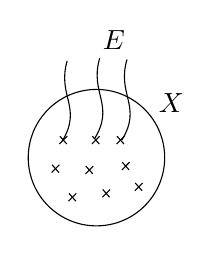
\begin{tikzpicture}[x=0.75pt,y=0.75pt,yscale=-1,xscale=1]
%uncomment if require: \path (0,300); %set diagram left start at 0, and has height of 300

%Flowchart: Connector [id:dp7499007648582767] 
\draw   (102,128.42) .. controls (102,110.26) and (116.72,95.55) .. (134.87,95.55) .. controls (153.02,95.55) and (167.74,110.26) .. (167.74,128.42) .. controls (167.74,146.57) and (153.02,161.29) .. (134.87,161.29) .. controls (116.72,161.29) and (102,146.57) .. (102,128.42) -- cycle ;
%Curve Lines [id:da20650999562395134] 
\draw    (118.28,120.59) .. controls (128.3,104.31) and (115.77,98.68) .. (120.78,81.77) ;
%Curve Lines [id:da9327641008081606] 
\draw    (133.93,119.34) .. controls (143.95,103.06) and (131.43,97.43) .. (136.43,80.52) ;
%Curve Lines [id:da6594075499360046] 
\draw    (147.08,119.97) .. controls (157.1,103.69) and (144.57,98.05) .. (149.58,81.15) ;
%Straight Lines [id:da13073640175251722] 
\draw    (117.25,118.09) -- (120.56,121.84) ;
%Straight Lines [id:da6620526994394944] 
\draw    (117.03,121.84) -- (120.78,118.09) ;

%Straight Lines [id:da8834541176981523] 
\draw    (132.9,118.09) -- (136.21,121.84) ;
%Straight Lines [id:da7510502290287235] 
\draw    (132.68,121.84) -- (136.43,118.09) ;

%Straight Lines [id:da44000068691517] 
\draw    (144.79,118.09) -- (148.11,121.84) ;
%Straight Lines [id:da8590400883175344] 
\draw    (144.57,121.84) -- (148.33,118.09) ;

%Straight Lines [id:da12268308784857629] 
\draw    (113.49,131.86) -- (116.81,135.62) ;
%Straight Lines [id:da22306917883937993] 
\draw    (113.27,135.62) -- (117.03,131.86) ;

%Straight Lines [id:da9728876585033619] 
\draw    (129.77,132.49) -- (133.08,136.24) ;
%Straight Lines [id:da23216656218706566] 
\draw    (129.55,136.24) -- (133.3,132.49) ;

%Straight Lines [id:da8478449055046726] 
\draw    (147.3,130.61) -- (150.61,134.37) ;
%Straight Lines [id:da7584484914378529] 
\draw    (147.08,134.37) -- (150.83,130.61) ;

%Straight Lines [id:da3145627797214947] 
\draw    (121.63,145.63) -- (124.94,149.39) ;
%Straight Lines [id:da696844406939886] 
\draw    (121.41,149.39) -- (125.17,145.63) ;

%Straight Lines [id:da4079053352483115] 
\draw    (137.91,143.76) -- (141.22,147.51) ;
%Straight Lines [id:da867418207840257] 
\draw    (137.69,147.51) -- (141.44,143.76) ;

%Straight Lines [id:da6401735618210065] 
\draw    (153.56,140.63) -- (156.87,144.38) ;
%Straight Lines [id:da7675951895008961] 
\draw    (153.34,144.38) -- (157.1,140.63) ;



% Text Node
\draw (163.62,96.13) node [anchor=north west][inner sep=0.75pt]   [align=left] {$X$};
% Text Node
\draw (136.7,66.07) node [anchor=north west][inner sep=0.75pt]   [align=left] {$E$};


\end{tikzpicture}
\end{figure}
\ei

\vspace{1cm} Roughly speaking, 
\bea
\text{observables} &= \text{functions on fields}\\
&=O(\sE) \ (\text{or certain homology})
\eea
\begin{eg}
Linear observables = distributions.
\end{eg}

The new structures come from the following fact:
\begin{itemize}
\item Given an open subset $U\subset X$, we can talk about
\bea \operatorname{Obs}(U)= \text{observables supported in U}.\eea

\begin{eg}
$\sE=C^\infty(X),\ p\in X$. Consider 
\bea \cO_1: \sE \ra \bR\eea
where $\cO_1(f)=f(p)^m, \ \forall f\in \sE$. $\cO_1$ is an observable supported in any open neighborhood of $p$.
\end{eg}

\item Let $\sE(U)=\Gamma(U,E)$. Then 
\bea
\operatorname{Obs}(U)=\text{functions on }  \sE(U).
\eea

\item The new structure is the \textbf{factorization product / operator product expansion (OPE)}. Given disjoint open subsets $U_i \subset V$, their disjoint union $\coprod_i U_i \subset V$, we have a map (factorization product):
\bea
\bigotimes_i \operatorname{Obs}(U_i)\mapsto \operatorname{Obs}(V).
\eea

\item Intuitively, if $\sE(U)$ is restricted to $\sE(U_i)$, then dually $O(\sE(U_i))\mapsto O(\sE(U))$.
Naively, we can {\em multiply} those {\em functions}, then we get
\bea
\bigotimes_i \operatorname{Obs}(U_i)\mapsto \operatorname{Obs}(V).
\eea
This, however, requires further {\em quantum corrections} in which fields in $U_i$'s may {\em talk} to each other.
\end{itemize}


\begin{eg}[Topological Quantum Mechanics]
In topological QFT, $\operatorname{Obs}(U)$ only depends on the topology of U.
Consider $\operatorname{dim} X=1$ and $\operatorname{Obs}(U)=A$ for a contractible open interval $U$. 

\begin{figure}[!htpb]\centering
\tikzset{every picture/.style={line width=0.75pt}} %set default line width to 0.75pt        

\begin{tikzpicture}[x=0.75pt,y=0.75pt,yscale=-1,xscale=1]
%uncomment if require: \path (0,300); %set diagram left start at 0, and has height of 300

%Straight Lines [id:da6858804075591907] 
\draw    (370,108.54) -- (559.34,108.54) ;
%Straight Lines [id:da31596934900875695] 
\draw    (373.66,196.97) -- (563,196.97) ;
%Straight Lines [id:da32970695145900697] 
\draw    (469.7,128.89) -- (469.7,164.09) ;
\draw [shift={(469.7,166.09)}, rotate = 270] [color={rgb, 255:red, 0; green, 0; blue, 0 }  ][line width=0.75]    (10.93,-3.29) .. controls (6.95,-1.4) and (3.31,-0.3) .. (0,0) .. controls (3.31,0.3) and (6.95,1.4) .. (10.93,3.29)   ;

% Text Node
\draw (434.14,106.54) node   [align=left] {{\huge ( \ \ \ \ \ )}};
% Text Node
\draw (495.55,107.24) node   [align=left] {{\huge ( \ \ \ \ \ )}};
% Text Node
\draw (469.6,196.37) node   [align=left] {{\huge ( \ \ \ \ \ \ \ \ \ \ \ \ )}};
% Text Node
\draw (426.75,78.64) node [anchor=north west][inner sep=0.75pt]   [align=left] {$U_1$};
% Text Node
\draw (487.25,78.64) node [anchor=north west][inner sep=0.75pt]   [align=left] {$U_2$};
% Text Node
\draw (463.53,171.38) node [anchor=north west][inner sep=0.75pt]   [align=left] {$V$};

\end{tikzpicture}
\end{figure}

\noindent We have a topological quantum mechanics (QM) with maps
\bea
\operatorname{Obs}(U_1)\otimes \operatorname{Obs}(U_2) \mapsto \operatorname{Obs}(V)
\eea
or equivalently,
\bea
A \otimes A \mapsto A
\eea
\end{eg}
\noindent We find an \textbf{associative algebra}!


\subsection*{Algebraic structure}
Consider two operators are placed at two different points on a line. When one operator approaches closely the other, the algebraic structure of the topology of the line comes from the homology group
\bea
H_{\bd} (\bR-\lcb 0\rcb)=H_0 (\bR-\lcb 0\rcb)= \bZ_{\text{Left}} \oplus \bZ_{\text{Right}}
\eea
which leads to left and right multiplications.

{\em Associativity} comes from further consistency:
\begin{figure}[!htpb]\centering
\tikzset{every picture/.style={line width=0.6pt}} %set default line width to 0.75pt        

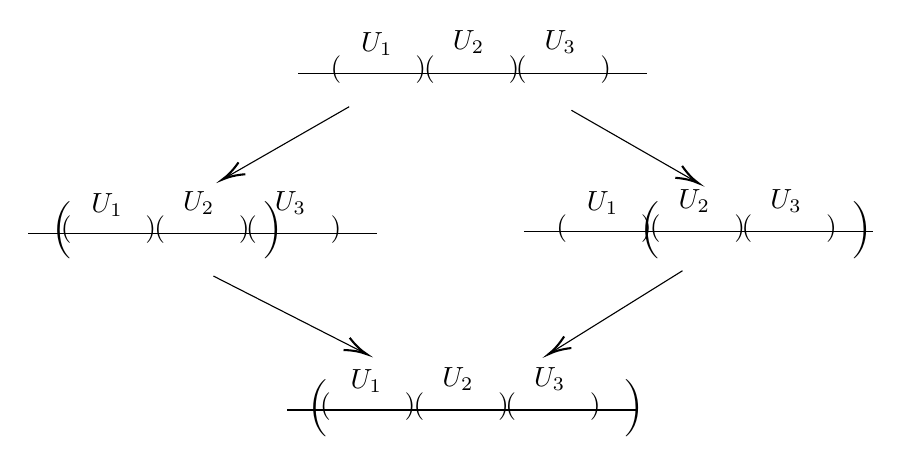
\begin{tikzpicture}[x=0.75pt,y=0.75pt,yscale=-1,xscale=1]
%uncomment if require: \path (0,300); %set diagram left start at 0, and has height of 300

%Straight Lines [id:da5543604292457156] 
\draw    (141,36.09) -- (309.24,36.09) ;
%Straight Lines [id:da4901487194099099] 
\draw    (11,113.41) -- (179.24,113.41) ;
%Straight Lines [id:da1721642744801426] 
\draw    (249.76,112.56) -- (418,112.56) ;
%Straight Lines [id:da22802491317770257] 
\draw    (135.9,198.38) -- (304.14,198.38) ;
%Straight Lines [id:da5450171031412938] 
\draw    (165.64,52.24) -- (106.2,86.36) ;
\draw [shift={(104.47,87.36)}, rotate = 330.14] [color={rgb, 255:red, 0; green, 0; blue, 0 }  ][line width=0.75]    (10.93,-3.29) .. controls (6.95,-1.4) and (3.31,-0.3) .. (0,0) .. controls (3.31,0.3) and (6.95,1.4) .. (10.93,3.29)   ;
%Straight Lines [id:da32782364610967507] 
\draw    (272.7,53.94) -- (332.15,88.06) ;
\draw [shift={(333.88,89.06)}, rotate = 209.86] [color={rgb, 255:red, 0; green, 0; blue, 0 }  ][line width=0.75]    (10.93,-3.29) .. controls (6.95,-1.4) and (3.31,-0.3) .. (0,0) .. controls (3.31,0.3) and (6.95,1.4) .. (10.93,3.29)   ;
%Straight Lines [id:da776515361469394] 
\draw    (100.22,133.81) -- (172.36,170.57) ;
\draw [shift={(174.14,171.48)}, rotate = 207] [color={rgb, 255:red, 0; green, 0; blue, 0 }  ][line width=0.75]    (10.93,-3.29) .. controls (6.95,-1.4) and (3.31,-0.3) .. (0,0) .. controls (3.31,0.3) and (6.95,1.4) .. (10.93,3.29)   ;
%Straight Lines [id:da4544384801263339] 
\draw    (326.23,131.26) -- (263.36,170.42) ;
\draw [shift={(261.66,171.48)}, rotate = 328.09] [color={rgb, 255:red, 0; green, 0; blue, 0 }  ][line width=0.75]    (10.93,-3.29) .. controls (6.95,-1.4) and (3.31,-0.3) .. (0,0) .. controls (3.31,0.3) and (6.95,1.4) .. (10.93,3.29)   ;

% Text Node
\draw (155.46,26.32) node [anchor=north west][inner sep=0.75pt]   [align=left] {( \ \ \ \ \ \ \ )};
% Text Node
\draw (200.5,26.32) node [anchor=north west][inner sep=0.75pt]   [align=left] {( \ \ \ \ \ \ \ )};
% Text Node
\draw (244.68,26.32) node [anchor=north west][inner sep=0.75pt]   [align=left] {( \ \ \ \ \ \ \ )};
% Text Node
\draw (170.16,15.27) node [anchor=north west][inner sep=0.75pt]   [align=left] {$U_1$};
% Text Node
\draw (214.35,14.42) node [anchor=north west][inner sep=0.75pt]   [align=left] {$U_2$};
% Text Node
\draw (258.53,14.42) node [anchor=north west][inner sep=0.75pt]   [align=left] {$U_3$};
% Text Node
\draw (25.46,103.64) node [anchor=north west][inner sep=0.75pt]   [align=left] {( \ \ \ \ \ \ \ )};
% Text Node
\draw (70.49,103.64) node [anchor=north west][inner sep=0.75pt]   [align=left] {( \ \ \ \ \ \ \ )};
% Text Node
\draw (114.68,103.64) node [anchor=north west][inner sep=0.75pt]   [align=left] {( \ \ \ \ \ \ \ )};
% Text Node
\draw (40.16,92.59) node [anchor=north west][inner sep=0.75pt]   [align=left] {$U_1$};
% Text Node
\draw (84.34,91.74) node [anchor=north west][inner sep=0.75pt]   [align=left] {$U_2$};
% Text Node
\draw (128.53,91.74) node [anchor=north west][inner sep=0.75pt]   [align=left] {$U_3$};
% Text Node
\draw (264.22,102.79) node [anchor=north west][inner sep=0.75pt]   [align=left] {( \ \ \ \ \ \ \ )};
% Text Node
\draw (309.26,102.79) node [anchor=north west][inner sep=0.75pt]   [align=left] {( \ \ \ \ \ \ \ )};
% Text Node
\draw (353.44,102.79) node [anchor=north west][inner sep=0.75pt]   [align=left] {( \ \ \ \ \ \ \ )};
% Text Node
\draw (278.92,91.74) node [anchor=north west][inner sep=0.75pt]   [align=left] {$U_1$};
% Text Node
\draw (323.11,90.89) node [anchor=north west][inner sep=0.75pt]   [align=left] {$U_2$};
% Text Node
\draw (367.29,90.89) node [anchor=north west][inner sep=0.75pt]   [align=left] {$U_3$};
% Text Node
\draw (150.37,188.61) node [anchor=north west][inner sep=0.75pt]   [align=left] {( \ \ \ \ \ \ \ )};
% Text Node
\draw (195.4,188.61) node [anchor=north west][inner sep=0.75pt]   [align=left] {( \ \ \ \ \ \ \ )};
% Text Node
\draw (239.58,188.61) node [anchor=north west][inner sep=0.75pt]   [align=left] {( \ \ \ \ \ \ \ )};
% Text Node
\draw (165.06,177.56) node [anchor=north west][inner sep=0.75pt]   [align=left] {$U_1$};
% Text Node
\draw (209.25,176.71) node [anchor=north west][inner sep=0.75pt]   [align=left] {$U_2$};
% Text Node
\draw (253.43,176.71) node [anchor=north west][inner sep=0.75pt]   [align=left] {$U_3$};
% Text Node
\draw (21.2,96.76) node [anchor=north west][inner sep=0.75pt]   [align=left] {{\huge ( \ \ \ \ \ \ \ \ \ \ )}};
% Text Node
\draw (304.9,96.76) node [anchor=north west][inner sep=0.75pt]   [align=left] {{\huge ( \ \ \ \ \ \ \ \ \ \ )}};
% Text Node
\draw (144.88,182.24) node [anchor=north west][inner sep=0.75pt]   [align=left] {{\huge ( \ \ \ \ \ \ \ \ \ \ \ \ \ \ \ \ )}};
\end{tikzpicture}
\end{figure}
\bea
\RA (a\cdot b)\cdot c= a\cdot (b\cdot c).
\eea

\begin{eg}[Chiral QFT] $\operatorname{dim }X=2$ (a plane). 
\begin{figure}[!htpb]\centering


\tikzset{every picture/.style={line width=0.75pt}} %set default line width to 0.75pt        

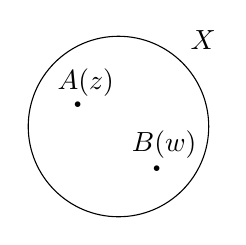
\begin{tikzpicture}[x=0.75pt,y=0.75pt,yscale=-1,xscale=1]
%uncomment if require: \path (0,300); %set diagram left start at 0, and has height of 300

%Shape: Ellipse [id:dp8384382557053032] 
\draw   (66.98,120.35) .. controls (66.98,96.34) and (86.45,76.87) .. (110.46,76.87) .. controls (134.48,76.87) and (153.94,96.34) .. (153.94,120.35) .. controls (153.94,144.37) and (134.48,163.83) .. (110.46,163.83) .. controls (86.45,163.83) and (66.98,144.37) .. (66.98,120.35) -- cycle ;

% Text Node
\draw (79.83,91.45) node [anchor=north west][inner sep=0.75pt]   [align=left] {$A(z)$};
% Text Node
\draw (115.66,121.35) node [anchor=north west][inner sep=0.75pt]   [align=left] {$B(w)$};
% Text Node
\draw (85.82,107.186) node [anchor=north west][inner sep=0.75pt]   [align=left] {{\Huge .}};
% Text Node
\draw (123.79,137.86) node [anchor=north west][inner sep=0.75pt]   [align=left] {{\Huge .}};
% Text Node
\draw (144,73) node [anchor=north west][inner sep=0.75pt]   [align=left] {$X$};
\end{tikzpicture}

\end{figure}

\noindent In holomorphic coordinates, when an operator approach (wind around) the other on $X$, the winding number can be kept track in terms of their Laurent modes:
\bea 
A(z)B(w)=\sum_{m\in \bZ}\frac{\lb A_{(m)}B\rb (w)}{(z-w)^{m+1}}.
\eea
We find $\infty$-many ``product'' (binary operation) $\lcb A_{(m)}B \rcb$. Observable algebras then give rise to \textbf{vertex algebras}.
\end{eg}

These are developed in the works of:
\begin{itemize}
    \item Beilinson-Drinfeld
    \begin{itemize}
        \item developed factorization algebra to formulate two-dimensional chiral conformal field theory (CFT)
        \item introduced the notion of {\em chiral homology} (generalize {\em Hodge homology} in one dimension)
    \end{itemize}
    \item Costello-Guilliam
    \begin{itemize}
        \item construction of factorization algebras from perturbative renormalization theory, in the \textbf{Batalin-Vilkovisky (BV) formalism} (generalize BRST formalism in gauge theory).
    \end{itemize}
\end{itemize}

%\begin{rem} The geometrical study of QFT are related to index theory: 1-dim. (Atiyah-Singer index theory), 2-dim. (chiral index theory on loop space). (see later) \end{rem}

\subsection*{BV formalism and homological integration}
    \bea \int \ =\ \text{homology}\eea
\begin{itemize}
    \item \underline{Calculus revisited}\\
    Let $M$ be a compact oriented manifold of $\operatorname{dim} M=n$. Many constructions of integration on manifolds can be understood from de Rham complex
    $\lb \Omega^\bd(M), d\rb$. Consider the integration map 
    \bea
    \int_M: \Omega^\bd(M)&\ra \bR\\
    \alpha\in \Omega^n(M) &\mapsto \int_M \alpha\eea
    Observe that the $n$-th de Rham cohomology group
    $H^n_{dR}(M) =\bR$
    \bea
    \RA\ \int_M \ = \ H^n_{dR} \ \lb
    \stackrel{n\ra\infty}{\leadsto}\ ? \text{ in QFT, interesting problem?}\rb\eea
    The integration map is now
    \bea
    \Omega^n(M) &\ra H^n_{dR}(M)\\
    \alpha &\mapsto [\alpha].
    \eea
    This means that we can learn calculus by the algebraic structure on de Rham complex, even we do not know anything about measure theory.
    
    \item \underline{BV approach}\\
    Define \textbf{polyvector fields}
    \bea 
    \operatorname{PV}^\bd(M) =\bigoplus_k \operatorname{PV}^k(M)= \bigoplus_k \Gamma \lb M,\ \bigw^k TM\rb.
     \eea
    Let $\Omega$ be a fixed volume form on $M$. We can naturally identify
    \bea
    \operatorname{PV}^k(M) &\lra \Omega ^{n-k}(M)\\
    \mu &\lra \mu \lrcorner \Omega
    \eea
    Locally, if $\Omega=e^\varphi dx^1\wedge \cdots \wedge dx^n$, $\mu=\mu^{i_1\cdots i_k} \partial_{i_1}\wedge \cdots \wedge \partial_{i_k}$, then
    \bea \mu \lrcorner\Omega= \sum \pm \mu^{i_1\cdots i_k} e^\varphi dx^1 \wedge \cdots \wedge \widehat{dx^{i_1}}\wedge \cdots \wedge\widehat{dx^{i_k}} \wedge \cdots \wedge dx^n. \eea
    
    The identification above leads to 
    \begin{figure}[!htpb]\centering
\tikzset{every picture/.style={line width=0.75pt}} %set default line width to 0.75pt        

\begin{tikzpicture}[x=0.75pt,y=0.75pt,yscale=-1,xscale=1]
%uncomment if require: \path (0,300); %set diagram left start at 0, and has height of 300

%Straight Lines [id:da7418770892542212] 
\draw    (77,75) -- (108.33,75) ;
\draw [shift={(110.33,75)}, rotate = 180] [color={rgb, 255:red, 0; green, 0; blue, 0 }  ][line width=0.75]    (10.93,-3.29) .. controls (6.95,-1.4) and (3.31,-0.3) .. (0,0) .. controls (3.31,0.3) and (6.95,1.4) .. (10.93,3.29)   ;
%Straight Lines [id:da7789911226523776] 
\draw    (150,75) -- (181.33,75) ;
\draw [shift={(183.33,75)}, rotate = 180] [color={rgb, 255:red, 0; green, 0; blue, 0 }  ][line width=0.75]    (10.93,-3.29) .. controls (6.95,-1.4) and (3.31,-0.3) .. (0,0) .. controls (3.31,0.3) and (6.95,1.4) .. (10.93,3.29)   ;
%Straight Lines [id:da8825213733946038] 
\draw    (212,74) -- (243.33,74) ;
\draw [shift={(245.33,74)}, rotate = 180] [color={rgb, 255:red, 0; green, 0; blue, 0 }  ][line width=0.75]    (10.93,-3.29) .. controls (6.95,-1.4) and (3.31,-0.3) .. (0,0) .. controls (3.31,0.3) and (6.95,1.4) .. (10.93,3.29)   ;
%Straight Lines [id:da6853513626542171] 
\draw    (74,124) -- (105.33,124) ;
\draw [shift={(107.33,124)}, rotate = 180] [color={rgb, 255:red, 0; green, 0; blue, 0 }  ][line width=0.75]    (10.93,-3.29) .. controls (6.95,-1.4) and (3.31,-0.3) .. (0,0) .. controls (3.31,0.3) and (6.95,1.4) .. (10.93,3.29)   ;
%Straight Lines [id:da40948388226369414] 
\draw    (155,124) -- (186.33,124) ;
\draw [shift={(188.33,124)}, rotate = 180] [color={rgb, 255:red, 0; green, 0; blue, 0 }  ][line width=0.75]    (10.93,-3.29) .. controls (6.95,-1.4) and (3.31,-0.3) .. (0,0) .. controls (3.31,0.3) and (6.95,1.4) .. (10.93,3.29)   ;
%Straight Lines [id:da4080909117329181] 
\draw    (207,124) -- (238.33,124) ;
\draw [shift={(240.33,124)}, rotate = 180] [color={rgb, 255:red, 0; green, 0; blue, 0 }  ][line width=0.75]    (10.93,-3.29) .. controls (6.95,-1.4) and (3.31,-0.3) .. (0,0) .. controls (3.31,0.3) and (6.95,1.4) .. (10.93,3.29)   ;

% Text Node
\draw (83,58) node [anchor=north west][inner sep=0.75pt]   [align=left] {$d$};
% Text Node
\draw (191,63) node [anchor=north west][inner sep=0.75pt]   [align=left] {$\cdots$};
% Text Node
\draw (157,58) node [anchor=north west][inner sep=0.75pt]   [align=left] {$d$};
% Text Node
\draw (219,57) node [anchor=north west][inner sep=0.75pt]   [align=left] {$d$};
% Text Node
\draw (47,66.4) node [anchor=north west][inner sep=0.75pt]    {$\Omega ^{0}$};
% Text Node
\draw (121,65.4) node [anchor=north west][inner sep=0.75pt]    {$\Omega ^{1}$};
% Text Node
\draw (249,64.4) node [anchor=north west][inner sep=0.75pt]    {$\Omega ^{n}$};
% Text Node
\draw (190,112) node [anchor=north west][inner sep=0.75pt]   [align=left] {$\cdots$};
% Text Node
\draw (41,115.4) node [anchor=north west][inner sep=0.75pt]    {$PV^{n}$};
% Text Node
\draw (81,103.4) node [anchor=north west][inner sep=0.75pt]    {$\Delta $};
% Text Node
\draw (163,105.4) node [anchor=north west][inner sep=0.75pt]    {$\Delta $};
% Text Node
\draw (216,104.4) node [anchor=north west][inner sep=0.75pt]    {$\Delta $};
% Text Node
\draw (109,113.4) node [anchor=north west][inner sep=0.75pt]    {$PV^{n-1}$};
% Text Node
\draw (241,113.4) node [anchor=north west][inner sep=0.75pt]    {$PV^{0}$};
% Text Node
\draw (61.81,87.57) node [anchor=north west][inner sep=0.75pt]  [rotate=-88.54,xslant=0.03]  {$\cong $};
% Text Node
\draw (133.81,87.57) node [anchor=north west][inner sep=0.75pt]  [rotate=-88.54,xslant=0.03]  {$\cong $};
% Text Node
\draw (263.81,87.57) node [anchor=north west][inner sep=0.75pt]  [rotate=-88.54,xslant=0.03]  {$\cong $};
% Text Node
\draw (286.14,46.01) node [anchor=north west][inner sep=0.75pt]  [font=\Large,rotate=-28.13]  {$\xrightarrow{\ \ \int \ \ }$};
% Text Node
\draw (269.44,119.51) node [anchor=north west][inner sep=0.75pt]  [font=\Large,rotate=-332.79]  {$\xrightarrow[   \ \int_{\text{BV}}\ ]{}$};
% Text Node
\draw (318,86.4) node [anchor=north west][inner sep=0.75pt]    {$\bR$};
\end{tikzpicture}
\end{figure}

where
$\Delta: \operatorname{PV}^k \ra \operatorname{PV}^{k-1}$ is a divergence operator with respect to $\Omega$ ($\Delta$ is called \textbf{BV operator}) and $\int_{\operatorname{BV}}$ is the BV integration.

\begin{eg}
$\Delta: \operatorname{PV}^1=\operatorname{Vect}(M) \ra \operatorname{PV}^0=C^\infty(M)$ is the usual divergence.
\end{eg}

The BV integration is a map:
\bea \int_{\operatorname{BV}}: \operatorname{PV}^0 &\ra \bR\\
f &\mapsto \int f\Omega
\eea

Homologically $\int_{\operatorname{BV}}\cong H^0_{\operatorname{BV}}$.
\begin{itemize}
    \item Here ``dim. $M$'' does not appear
    \item In $\infty$-dimensions, renormalization helps to construct $\Delta$ which leads to \textbf{homological integration }
\end{itemize}

\item \underline{Explicit form of $\Delta$}\\
Locally in $U$, let $\lcb x_i\rcb$ be local coordinates, the volume form be $\Omega=e^{f(x)}dx^1\wedge \cdots \wedge dx^n$. Introduce the vector fields $\partial_i=\frac{\partial}{\partial x_i}$, then the polyvector field is \bea \operatorname{PV}(U)=C^\infty(U) [\partial_1, \cdots, \partial_n],\eea
where $\partial_i$'s are anticommuting: $\partial_i \partial_j =- \partial_j \partial_i$. 
Let us write $\theta_i=\partial_i$ (\textit{note}: this is a vector field, NOT an differential operator), then a local section $\mu\in \operatorname{PV}(X)$ can be written as a function of $x^i$, $\theta_i$:
\bea
\mu=\mu (x^i, \theta_i)
\eea
with $x^ix^j=x^j x^i$ and $\theta_i \theta_j =- \theta_j \theta_i$.
Let $\frac{\partial}{\partial x^i}$ be the derivative with respect to $x^i$  and $\frac{\partial}{\partial \theta_i}$ be the derivative with respect to $\theta_i$ (from the left). Then the BV operator is given locally by 
\bea
\Delta = \sum_i \frac{\partial}{\partial x^i} \frac{\partial}{\partial \theta_i}
+\sum_i (\partial_i f) \frac{\partial}{\partial \theta_i}
\eea
which looks like a second order operator. This is in contrast with de Rham differential $d$, which is a first order differential
operator. Note that the first term looks like a Laplacian, but it is NOT. $\theta_i$ is an odd variable.

\begin{eg}[$\frac{\partial}{\partial \theta_i}$ operator]
\bea\frac{\partial}{\partial \theta_1}(\theta_1\theta_2)=\theta_2,\\
\frac{\partial}{\partial \theta_1}(\theta_2\theta_1)=- \frac{\partial}{\partial \theta_1}(\theta_1\theta_2)=-\theta_2.
\eea
\end{eg}

\begin{eg}[Singularity theory]
Consider the $n$-th dimensional complex space $\bC^n$. Let $f: \bC^n\ra \bC$ be a polynomial with an isolated critical pint at 0:
\bea \operatorname{Crit}(f)=\lcb 0\rcb.\eea
We consider holomorphic/polynomial polyvector fields
\bea \cA =\bC[z^i, \theta_i], \quad
\theta_i \theta_j =- \theta_j \theta_i.\eea
Let
\bea \Delta=\hbar \sum_{i=1}^n \frac{\partial}{\partial z^i} \frac{\partial}{\partial \theta_i}
+\sum_i (\partial_i f) \frac{\partial}{\partial \theta_i}. \eea
Then
\begin{itemize}
    \item Quantum observable $\operatorname{Obs}^q=H^\bd (\cA[[\hbar]],\Delta)\cong$ Brieskorn lattice.
    \item 
    $\hbar$-filtration = Hodge filtration.
    \item BV-integration gives rise to evaluation map on observable $\lan \cO\ran=\int_{\mathscr{L}}\cO e^{f/\hbar}$ (an oscillatory integral) where $\mathscr{L}$ is Lefschetz timble.
\end{itemize}

\end{eg}

















\end{itemize}

\end{document}
